\hypertarget{expresiones-booleanas}{%
\section{Boolean expressions}\label{expresiones-booleanas}}

\index{booleana, expresión} \index{expresión!booleana}
\index{lógico, operador} \index{operador!lógico}

A \emph{boolean expression} is a expression that can be true (\texttt{True}) or false (\texttt{False}). The following examples use the \texttt{==} operator, which compares two operands and returns
\texttt{True} if they are equal and \texttt{False} otherwise:

\begin{Verbatim}[frame=single]
>>> 5 == 5
  True
>>> 5 == 6
  False
\end{Verbatim}

\texttt{True} and \texttt{False} are special values that belong to the \texttt{bool\ (boolean)} type; they are not strings:

\index{True, valor especial} \index{False, valor especial}
\index{valor especial!True} \index{valor especial!False}
\index{booleano, tipo} \index{tipo!booleano}

\begin{Verbatim}[frame=single]
>>> type(True)
  <class 'bool'>
>>> type(False)
  <class 'bool'>
\end{Verbatim}

The \texttt{==} operator is one of the \emph{comparison operators}; the other comparison operators (or relational operators) are:

\begin{python}[frame=single]
x != y               # x is different from y
x > y                # x is greater than y
x < y                # x is less than y
x >= y               # x is greater than or equal to y
x <= y               # x is less than or equal to y
x is y               # x is the same as y
x is not y           # x is not the same as y
\end{python}

Although these operations are probably familiar to you, the symbols in Python are different from the mathematical symbols used to perform the same operations. A very common mistake is to use just an equals symbol (\texttt{=}) instead of the double equals symbol (\texttt{==}). Remember that \texttt{=} is an assignment operator, and \texttt{==} is a comparison operator. There is no such thing as \texttt{=\textless{}} or \texttt{=\textgreater{}}.

\index{comparación!operador} \index{operador!comparación}


Comparison operators (or relational operators) work on strings. To see if two strings are equal:

\begin{python}[frame=single]
if word == 'banana':
    print('Everything is fine, banana.')
\end{python}
%
Other relational operations are useful for putting words in alphabetical order:

\begin{python}[frame=single]
if word < 'banana':
    print('Your word, ' + word + ', comes before banana.')
elif word > 'banana':
    print('Your word, ' + word + ', comes before banana.')
else:
    print('Everything is fine, banana.')
\end{python}
%
Python doesn't handle uppercase and lowercase letters the same way people do. Use ASCII code to compare letters. ASCII is an English acronym for the American Standard Code for Information Interchange. In Figure \ref{fig:ASCII} you can see (part of) the numbers that the ASCII code assigns to each letter. We can see that all uppercase letters come before all lowercase letters, so the word Pineapple comes before banana.

\begin{Verbatim}[frame=single]
>>> "Pineapple" < "banana"
  True
\end{Verbatim}


\begin{figure}
    \centering
    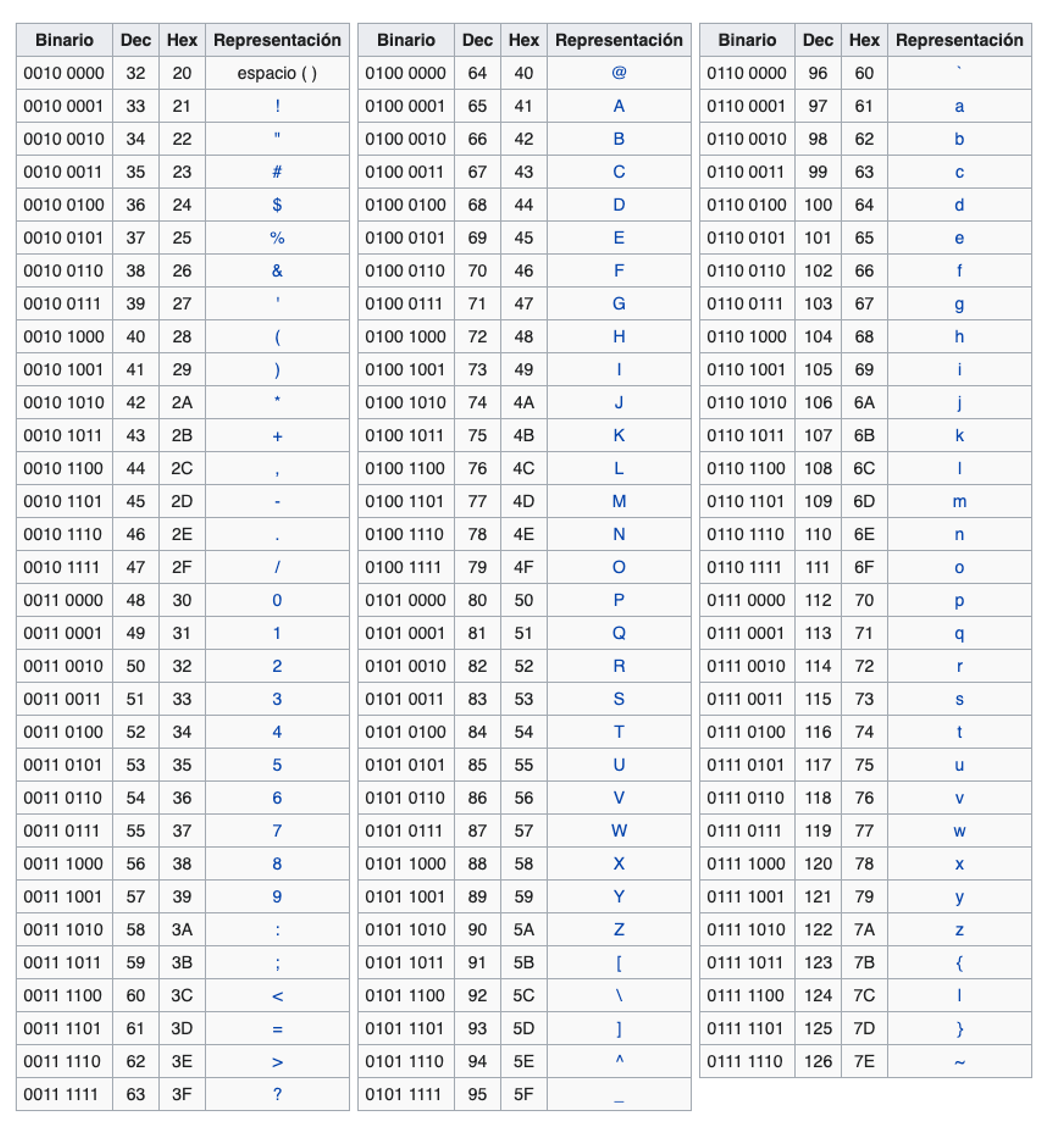
\includegraphics[width=190px]{images/ASCII.png}
    \caption{The ASCII code}
    \label{fig:ASCII}
\end{figure}

Python offers \texttt{ord} and \texttt{chr} functions to find out the ASCII code of letters or vice versa (the letter that corresponds to a code):

\begin{Verbatim}[frame=single]
>>> ord("a")
  97
>>> ord("W")
  87
>>> chr(97)
  'a'
\end{Verbatim}


\hypertarget{operadores-luxf3gicos}{%
\section{Logical operators}\label{operadores-luxf3gicos}}

\index{lógico, operador} \index{operador!lógico}

There are three \emph{logical operators}: \texttt{and}, \texttt{or} and \texttt{not}. The semantic meaning of these operations is similar to their meaning in English. For example,

\texttt{x\ \textgreater{}\ 0\ and\ x\ \textless{}\ 10}

is true only when \texttt{x} is greater than 0 \emph{and} less than 10.

\index{and, operador} \index{or, operador} \index{not, operador}
\index{operador!and} \index{operador!or} \index{operador!not}

\texttt{n\%2\ ==\ 0\ or\ n\%3\ ==\ 0} 

is true if \emph{any} of the conditions is true, that is, if the number is divisible by 2 \emph{or} by 3.

Finally, the \texttt{not} operator negates a Boolean expression, so

\texttt{not\ (x\ >\ y)} 

is true if \texttt{x\ >\ y} is false; that is, if \texttt{x} is less than or equal to \texttt{y}.

Strictly speaking, the operands of logical operators should be boolean expressions, but Python isn't very strict. Any non-zero number is interpreted as \pythoninline{True}.

\begin{Verbatim}[frame=single]
>>> 18 and True
  True
\end{Verbatim}

This flexibility can be helpful, but there are some subtleties to that kind of usage that can be confusing. You may want to avoid using it in this way until you are quite sure what you are doing.

\hypertarget{ejecuciuxf3n-condicional}{%
\section{Conditional execution}\label{ejecuciuxf3n-condicional}}

\index{condicional!sentencia} \index{sentencia!condicional}
\index{if, sentencia} \index{sentencia!if} \index{condicional!ejecución}

In order to write useful programs, we usually need the ability to test for conditions and change the behavior of the program accordingly. \texttt{Conditional\ statements} (or just \texttt{if-then} or \texttt{if-elif-else}) provide us with that capability. The simplest form is the \texttt{if} statement:

\begin{python}[frame=single]
if x > 0 :
    print('x is positive')
\end{python}

The Boolean expression after the \texttt{if} is called the \emph{condition} and is terminated by a colon (:), and the line(s) below the \texttt{if} statement are indented (that is, they have a tab or several blank spaces at the beginning).

If the logical condition is true, the indented statement will be executed. If the condition is false, the indented statement will be skipped.

\index{condición} \index{compuesta, instrucción}
\index{instrucción!compuesta}

The \texttt{if} statement has the same structure as the definition
of functions or \texttt{for} loops\footnote{We will study functions and loops in later topics.}. The statement consists of a header line ending with the colon character (:) followed by an indented block. Statements of this type are called \emph{compound statements}, because
they span multiple lines.

There is no limit to the number of statements that can appear in the
body, but there must be at least one. Occasionally, it can be useful to have a body with no instructions (usually as a place reserved for code that hasn't been written yet). In that case, the \texttt{pass} instruction can be used, which does nothing.

\index{pass, sentencia} \index{sentencia!pass}

\begin{python}[frame=single]
if x < 0 :
    pass          # I need to manage negative values!
\end{python}

If you enter a \texttt{if} statement interactively at the Python console, the prompt will change its usual appearance to ellipses (\emph{\ldots{}}), to inform you that you are in the middle of a block of statements, like shown below:


\begin{Verbatim}[frame=single]
>>> x = 3
>>> if x < 10:
...    print('Small')
...
  Small
\end{Verbatim}

When using the Python interpreter, you must leave a blank line at the end of a block, otherwise Python will return an error:

\begin{Verbatim}[frame=single]
>>> x = 3
>>> if x < 10:
...    print('Small')
... print('Done')
  File "<stdin>", line 3
    print('Done')
        ^
SyntaxError: invalid syntax
\end{Verbatim}

A blank line at the end of a statement block is not necessary when writing and running a script, but it can improve the readability of your code.

\hypertarget{ejecuciuxf3n-alternativa}{%
\section{Alternative execution}\label{ejecuciuxf3n-alternativa}}

\index{ejecución alternativa} \index{else, palabra clave}
\index{palabra clave!else}

The second form of the \texttt{if} statement is the \emph{alternative execution}, in which there are two possibilities and the condition determines which of them will be executed. The syntax is similar to this:

\begin{python}[frame=single]
if x%2 == 0 :
    print('x is even')
else :
    print('x is odd')
\end{python}

If dividing \texttt{x} by 2 gives us a remainder of 0, then we know that \texttt{x} is even, and the program displays a message to that effect. If that condition is false, the second set of instructions is executed.

\begin{figure}[H]
\centering
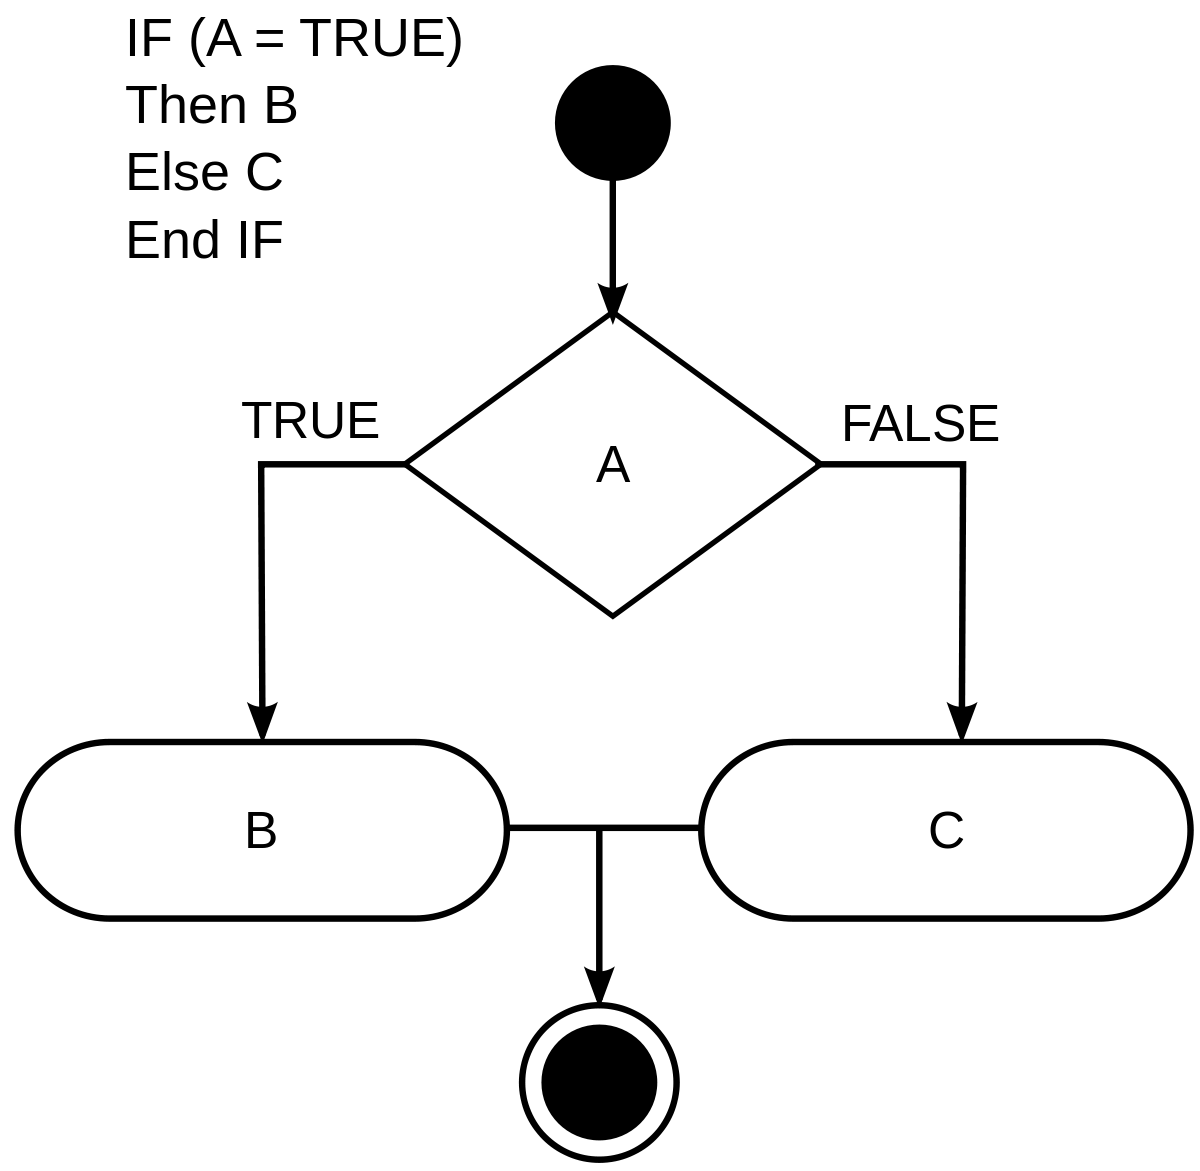
\includegraphics[width=180px]{images/if-eng.png}
\caption{If-Then-Else logic}
\label{fig:if}
\end{figure}

Since the condition must be true or false, only one of the alternatives will be executed. Alternatives are called \emph{branches}, since they are branches in the flow of execution.

\index{rama}

\hypertarget{condicionales-multiples-elif}{%
\section{Multiple conditionals
(elif)}\label{condicionales-multiples-elif}}

\index{encadenado, condicional} \index{condicional!encadenado}

Sometimes there are more than two possibilities, so we need more than two branches. One way to express an operation like that is to use a \emph{chained conditional}:

\begin{python}[frame=single]
if x < y:
    print('x is less than y')
elif x > y:
    print('x is greater than y')
else:
    print('x and y are equal')
\end{python}

\texttt{elif} is abbreviation for ``else if''. In this case also only one of the branches will be executed.

\begin{figure}[t]
\centering
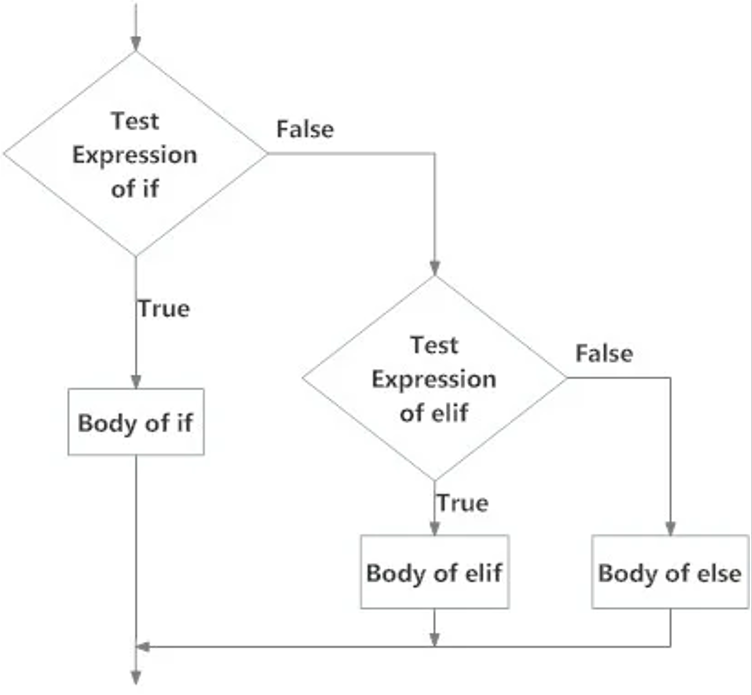
\includegraphics[width=250px]{images/elif-eng.png}
\caption{If-Then-Elif Logic}
\label{fig_elif}
\end{figure}

There is no limit to the number of \texttt{elif} expressions to use. If there is an \texttt{else} clause, it must come at the end, but it is not required to exist either.

\index{elif, palabra clave} \index{palabra clave!elif}

\begin{python}[frame=single]
if choice == 'a':
    print('Wrong answer')
elif choice == 'b':
    print('Correct answer')
elif choice == 'c':
    print('Almost, but not correct')
\end{python}

Each condition is checked in order. If the first is false, the next is checked, and so on. If one of them is true, the corresponding branch is executed, and the statement ends. Even if more than one condition is true, only the first one found is executed.

\hypertarget{condicionales-anidados}{%
\section{Nested conditionals}\label{condicionales-anidados}}

\index{anidado, condicional} \index{condicional!anidado}

A conditional can also be nested inside another. We could have written the above example of the three branches like this:

\begin{python}[frame=single]
if x == y:
    print('x and y are equal')
else:
    if x < y:
        print('x is less than y')
    else:
        print('x is greater than y')
\end{python}

The outer conditional contains two branches. The first branch executes a single statement. The second contains another \texttt{if} statement, which has its own two branches. Those two branches are both simple statements, but they could have been conditional statements as well.

\begin{figure}[H]
\centering
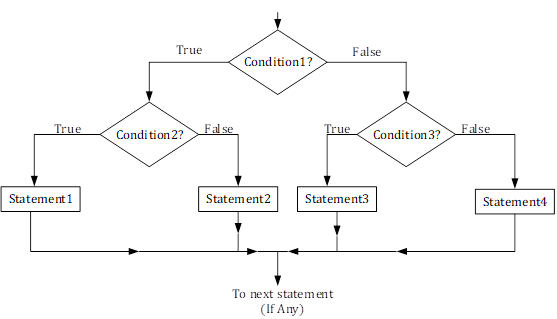
\includegraphics[width=350px]{images/nested-eng.png}
\caption{Nested If Statements}
\label{fig:nested}
\end{figure}

Although the indentation of the statements makes the structure clear, \emph{nested conditionals} can quickly become difficult to read. In general, it's a good idea to avoid them if you can. Logical operators often provide a way to simplify nested conditional statements. For example, the following code can be rewritten using a single conditional:

\begin{python}[frame=single]
if 0 < x:
    if x < 10:
        print('x is a positive number with a single digit.')
\end{python}

The \texttt{print} statement is executed only if both of the above conditions are met, so we can actually achieve the same effect with the \texttt{and} operator:

\begin{python}[frame=single]
if 0 < x and x < 10:
    print('x is a positive number with a single digit.')
\end{python}

\hypertarget{captura-de-excepciones-usando-try-y-except}{%
\section{Catching exceptions using try and except}\label{captura-de-excepciones-usando-try-y-except}}

Earlier we saw a code snippet where we used the \texttt{input} and \texttt{int} functions to read and parse an integer entered by the user. We also saw how unsafe it could be to do something like this:

\begin{Verbatim}[frame=single]
>>> speed = int(input("Enter a number: "))
Enter a number: r
Traceback (most recent call last):
  File "<pyshell>", line 1, in <module>
ValueError: invalid literal for int() with base 10: 'r'
\end{Verbatim}

When we are working with the Python interpreter, after the error
we just get the prompt again, so we think ``hey, I made a mistake!'', and continue with the next instruction.

However, if you write that code in a Python script and the error occurs, the script will stop immediately, displaying a ``traceback''. It will not execute the next statement.

\index{traceback}

Here is an example program to convert a temperature from degrees Fahrenheit to degrees Celsius:

\index{fahrenheit} \index{celsius} \index{conversión de temperatura}

\begin{python}
ent = input('Enter the Fahrenheit temperature:')
fahr = float(ent)
cel = (fahr - 32.0) * 5.0 / 9.0
print(cel)
\end{python}

If we run this code and give it invalid input, it will simply fail with a quite unfriendly error message:

\begin{Verbatim}[frame=single]
>>> %Run fahren.py
  Enter the Fahrenheit temperature:72
  22.2222222222
\end{Verbatim}

\begin{Verbatim}[frame=single]
>>> %Run fahren.py
  Enter the Fahrenheit temperature:fred
  Traceback (most recent call last):
  File "fahren.py", line 2, in <module>
    fahr = float(ent)
  ValueError: invalid literal for float(): fred
\end{Verbatim}

There are conditional execution structures within Python to handle these types of expected and unexpected errors, called ``try/except''. The idea of \texttt{try} and \texttt{except} is that if you know that a certain sequence of statements might cause a problem, you can add certain statements to be executed on failure. These extra statements (the except block) will be ignored if no error occurs.

You can think of the \texttt{try} and \texttt{except} feature of
Python as an ``insurance policy'' in a script.

We can rewrite our temperature converter like this:

\begin{python}
ent = input('Enter the Fahrenheit temperature:')
try:
    fahr = float(ent)
    cel = (fahr - 32.0) * 5.0 / 9.0
    print(cel)
except:
    print('Please enter a number')
\end{python}

Python begins by executing the sequence of statements in the \texttt{try} block. If all goes well, it will skip the entire \texttt{except} block and exit. If an exception occurs within the \texttt{try} block, Python will jump out of that block and execute the sequence of statements in the \texttt{except} block.

\begin{Verbatim}
>>> %Run fahren2.py
  Enter the Fahrenheit temperature:72
  22.2222222222
\end{Verbatim}

\begin{Verbatim}
>>> %Run fahren2.py
  Enter the Fahrenheit temperature:fred
  Please enter a number
\end{Verbatim}

Handling an exception with a \texttt{try} statement is called \emph{catching} an exception. In this example, the \texttt{except} clause displays an error message. In general, catching an exception gives you a chance to fix the problem, try again, or at least gracefully terminate the program.

\hypertarget{evaluaciuxf3n-en-cortocircuito-de-expresiones-luxf3gicas}{%
\section{Short-circuit evaluation of logical expressions}\label{evaluaciuxf3n-en-cortocircuito-de-expresiones-luxf3gicas}}

\index{cortocircuito}

When Python is processing a logical expression, such as \texttt{x\ >=\ 2\ and\ (x/y)\ >\ 2}, it evaluates the expression from left to right. Due to the definition of \texttt{and}, if \texttt{x} is less than 2, the expression \texttt{x\ >=\ 2} turns out to be \texttt{false}, so the entire expression already goes to return \texttt{false}, regardless of whether \texttt{(x/y)\ >\ 2} evaluates to \texttt{true} or \texttt{false}.

When Python detects that there is nothing to be gained by evaluating the rest of a logical expression, it stops evaluating it and does not compute the rest of the expression. When the evaluation of a logical expression stops because the final value is already known, this is known as \emph{short-circuiting} the evaluation (or lazy evaluation).

Although this may seem like a stretch, short-circuit operation reveals an ingenious technique known as \emph{guardian pattern}. Examine the following code statement in the Python interpreter:

\begin{Verbatim}[frame=single]
>>> x = 6
>>> y = 2
>>> x >= 2 and (x/y) > 2
  True
>>> x = 1
>>> y = 0
>>> x >= 2 and (x/y) > 2
  False
>>> x = 6
>>> y = 0
>>> x >= 2 and (x/y) > 2
  Traceback (most recent call last):
    File "<stdin>", line 1, in <module>
  ZeroDivisionError: division by zero
\end{Verbatim}

The third operation failed because Python tried to evaluate
\texttt{(x/y)} and \texttt{y} was zero, which causes a runtime error. But the second example \emph{did not} fail, because the first part of the expression \texttt{x\ >=\ 2} evaluated to \texttt{false}, so \texttt{(x/y)} did not run due to the \emph{short-circuit} rule, and no error occurred.

It is possible to build the logical expressions by strategically placing an evaluation as a \emph{guardian} just before the evaluation that would cause an error, as shown below:

\begin{Verbatim}[frame=single]
>>> x = 1
>>> y = 0
>>> x >= 2 and y != 0 and (x/y) > 2
  False
>>> x = 6
>>> y = 0
>>> x >= 2 and y != 0 and (x/y) > 2
  False
>>> x >= 2 and (x/y) > 2 and y != 0
  Traceback (most recent call last):
    File "<stdin>", line 1, in <module>
  ZeroDivisionError: division by zero
\end{Verbatim}

In the first logical expression, \texttt{x\ >=\ 2} is \texttt{false}, so evaluation stops at the \texttt{and}. In the second logical expression, \texttt{x\ >=\ 2} is \texttt{true}, but \texttt{y\ !=\ 0} is \texttt{false}, so \texttt{(x/y)} is never reached.

In the third logical expression, the \texttt{y\ !=\ 0} comes \emph{after} the calculation of \texttt{(x/y)}, so the expression fails with an error.

In the second expression, \texttt{y\ !=\ 0} acts as a \emph{guard} to ensure that \texttt{(x/y)} is only executed in case \texttt{y} is not zero.

\hypertarget{depuraciuxf3n}{%
\section{Debugging}\label{depuraciuxf3n}}

\index{depuración} \index{traceback}

The ``traceback'' that Python displays when an error occurs contain a lot of information, but can be overwhelming. The most useful parts are usually:
\begin{itemize}
\item
  What kind of error has occurred, and
\item
  Where has it happened?
\end{itemize}

Syntax errors are usually easy to spot, but can sometimes be confusing. Errors due to white space can be tricky, since spaces and tabs are invisible, and we tend to ignore them.

\index{espacio en blanco}

\begin{Verbatim}[frame=single]
>>> x = 5
>>>  y = 6
  File "<stdin>", line 1
    y = 6
    ^
IndentationError: unexpected indent
\end{Verbatim}

In this example, the problem is that the second line is indented by a space. But the error message points to \texttt{y}, which is misleading. In general, the error messages indicate where the problem has been discovered, but the real error could be in the previous code, sometimes in some previous line.

In general, error messages tell you where the problem was discovered, but often that's not exactly where it occurred.

\hypertarget{glosario_conditionals}{%
\section{Glossary}\label{glosario_conditionals}}

\begin{description}
\item[condition]
The boolean expression in a conditional statement that determines which branch will be executed.
\end{description}

\index{condición}

\begin{description}
\item[nested conditional]
A conditional statement that appears on one of the branches of another conditional statement.
\end{description}

\index{anidado, condicional} \index{condicional!anidado}

\begin{description}
\item[chained conditional]
A conditional statement with a series of alternative branches.
\end{description}

\index{encadenado, condicional} \index{condicional!encadenado}

\begin{description}
\item[short circuit]
When Python evaluates a logical expression piecewise and stops the evaluation process because it already knows the final value of the result without having to evaluate the rest of the expression.
\end{description}

\index{cortocircuito}

\begin{description}
\item[body]
The sequence of statements inside a compound statement.
\end{description}

\index{cuerpo}

\begin{description}
\item[boolean expression]
An expression whose value can be either \texttt{True} or \texttt{False}.
\end{description}

\index{booleana, expresión} \index{expresión!booleana}

\begin{description}
\item[comparison operators]
One of the operators used to compare two operands:
\texttt{==}, \texttt{!=}, \texttt{\textgreater{}}, \texttt{\textless{}},
\texttt{\textgreater{}=}, y \texttt{\textless{}=}.
\item[logical operator]
One of the operators that are combined in Boolean expressions:
\texttt{and}, \texttt{or}, and \texttt{not}.
\item[guardian pattern]
When we build a logical expression with additional comparisons to take advantage of short-circuiting.
\end{description}

\index{guardián, patrón} \index{patrón!guardián}

\begin{description}
\item[branch]
One of the alternative sequences of statements in a conditional statement.
\end{description}

\index{rama}

\begin{description}
\item[compound statement]
An instruction consisting of a header and a body. The header ends with a colon (:). The body is indented relative to the header.
\end{description}

\index{compuesta, sentencia} \index{sentencia!compuesta}

\begin{description}
\item[conditional statement]
An instruction that controls the flow of execution, depending on a certain condition.
\end{description}

\index{condicional!instrucción} \index{instrucción!condicional}

\begin{description}
\item[traceback]
A list of currently executing functions, which is displayed on the screen when an exception occurs.
\end{description}

\index{traceback}



\hypertarget{ejercicios}{%
\section*{Exercises}\label{ejercicios}}
\addcontentsline{toc}{section}{Exercises}

\begin{enumerate}
%\setlength{\itemindent}{1.3cm}
\setlength\itemsep{2em}

\item What result do the following expressions produce?

(a)  \pythoninline{True and not False}

(b) \pythoninline{True or not True}

(c) \pythoninline{True or True and False }

(d) \pythoninline{not True or not False }

(e) \pythoninline{True and not 0 }

(f) \pythoninline{52 < 52.3 }

(g) \pythoninline{1 + 52 < 52.3 }

(h) \pythoninline{4 \!= 4.0}

(i) \pythoninline{'peach' < 'apple'}

(j)  \pythoninline{'elephant' > 'Mouse'}



\respuesta{
a. True
b. True 
c. True 
d. True 
e. True
f. True
g. False
h. False
}

\item Write a Python expression that returns True if a given integer n is greater than 100 or less than 0.

\respuesta{
\pythoninline{(n > 100) or (n < 0)}
}

\item Write a Python expression that returns True if a given integer n is odd and in the interval [2, 16[.

\respuesta{\pythoninline{(n \% 2 == 0) and (n >=2 and n < 16)}}

\item Imagine that a and b are Boolean variables. Write expressions in Python that:

(a) returns True if and only if both variables are True

(b) returns True if and only if a is False

(c) returns True if and only if at least one of the variables is True.

\respuesta{
a. \pythoninline{a and b }

b. \pythoninline{not a }

c. \pythoninline{a or b}
}


\item Variables full and empty are variables of Boolean type. Write a Python expression that evaluates to True when at most one of the variables is True.

\respuesta{
\pythoninline{(full or empty) and not (full and empty)}
}

\item We want a camera to turn on automatically if the light level is below 0.01 lux or if the temperature is above zero, but not if both conditions are true. (You should assume that the function turn-camera-on has already been defined.) Your friend Anna says it has to be:


\begin{python}
if ((light<0.01) or (temp>0)) and  not ((light<0.01) and (temp>0)):
	turn_camera_on()
\end{python}

Your friend Maria says that it can also be written more simply using:

\begin{python}
if (light<0.01) != (temp>0.0):
	turn_camera_on()
\end{python}

Are they both right? why?


\respuesta{
Si! Imagina que L es \pythoninline{(light<0.01)} y T es \pythoninline{(temp>0.0)}. Podemos hacer una tabla de verdad:


\begin{tabular}{|l|l|l|l|l}
\hline
L & T & L!=T & L or T and not (L and T)  \\
\hline
True                      & True                      & False                        & False           \\
\hline
True                      & False                     & True                         & True        \\
\hline
False                     & True                      & True                         & True                     \\
\hline
False                     & False                     & False                        & False           \\
\hline
\end{tabular}
}


\item Complete the following table indicating which statement is executed based on the values of condition1, condition2, and condition3. Indicate with a \verb|-| when the condition is not evaluated.

\begin{python}
if condition1:
    if condition2:
        action1
    else:
        action2
else:
    if condition3:
        action3
    else:
        action4
\end{python}


\begin{tabular}{|l|l|l|l|}
\hline
condition1 & condition2 & condition3 & statement \\
\hline
\hline
           &            &            &             \\ \hline
           &            &            &        
          \\ \hline
                     &            &            &        
          \\ \hline
                     &            &            &        
          \\ \hline
\end{tabular}


\item \label{coords} Write a Python program that asks the user for the coordinates of two points in the plane, displaying on the screen the point that is closest to the origin.

\begin{itemize}
    \item Remember Pythagoras
    
    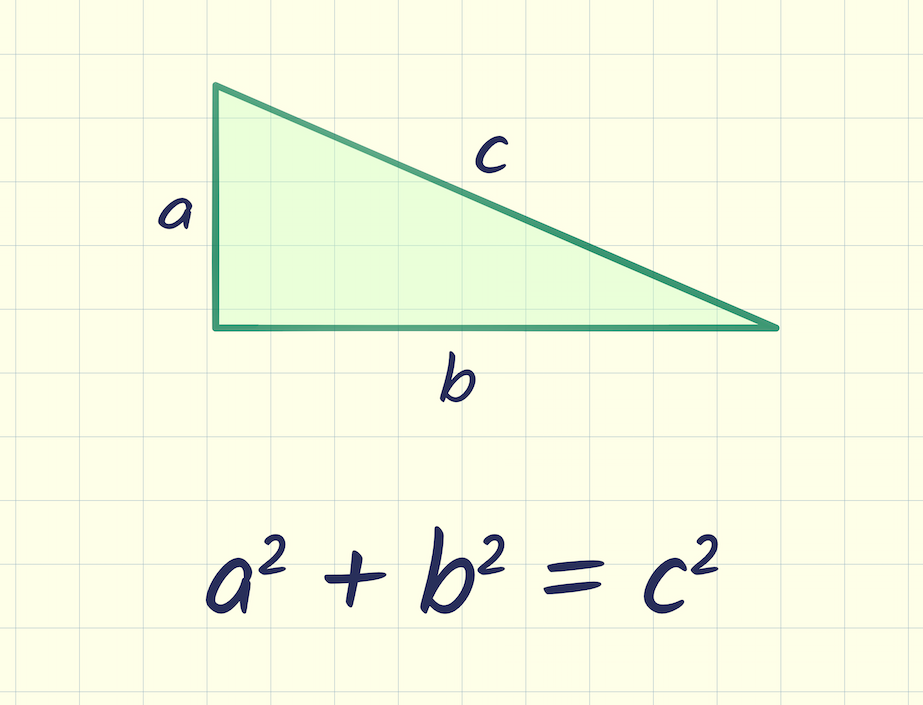
\includegraphics[width=0.3\textwidth]{images/pythagoras.png}
    \item The distance to the origin of the point (x, y) is the square root of the sum of the squares of its coordinates.
    \item To calculate the square root in Python we can use the function: math.sqrt():

\begin{Verbatim}[frame=single]
>>> import math
>>> math.sqrt(25)
5.0
>>> 
\end{Verbatim}
\end{itemize}

\begin{Verbatim}[frame=single, label={\em example test execution of the program}]
>>> %Run 
  x-coordinate of the 1st point in the plane: 2.5
  y-coordinate of the 1st point in the plane: 3.03
  x-coordinate of the 2nd point in the plane: 6
  y-coordinate of the 2nd point in the plane: 7.4
  The point (2.5,3.0) is the closest to the origin
>>> %Run 
  x-coordinate of the 1st point in the plane: 5
  y-coordinate of the 1st point in the plane: 9
  x-coordinate of the 2nd point in the plane: -2
  y-coordinate of the 2nd point in the plane: 1
  The point (-2.0,0.0) is the closest to the origin
>>> %Run 
  x-coordinate of the 1st point in the plane: 0
  y-coordinate of the 1st point in the plane: 0
  x-coordinate of the 2nd point in the plane: 0
  y-coordinate of the 2nd point in the plane: 0
  The distance to the origin is the same for both points
>>> %Run 
  x-coordinate of the 1st point in the plane: 1
  y-coordinate of the 1st point in the plane: 3
  x-coordinate of the 2nd point in the plane: 8
  y-coordinate of the 2nd point in the plane: -1
  The point (1.0,3.0) is the closest to the origin
\end{Verbatim}
 
In these 3 executions we are testing:

\begin{itemize}
    \item first point (quadrant I), second point (quadrant I)
    \item first point (quadrant I), second point (quadrant II)
    \item both points are the origin
    \item first point (quadrant I), second point (quadrant IV)
\end{itemize}

\begin{figure}[H]
\centering
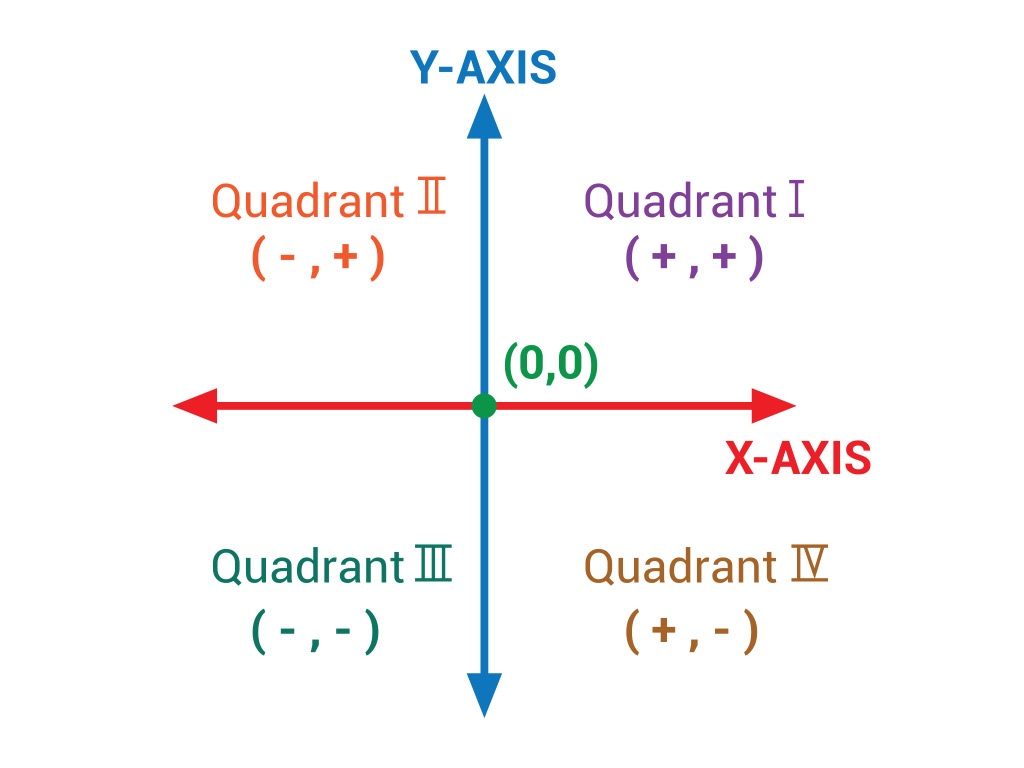
\includegraphics[width=0.5\textwidth]{images/quadrant.jpg}
\caption{Coordinate plane}
\label{fig:if}
\end{figure}

 

If we want to try all the combinations of the quadrants. What other tests do we have to run?

\item In an electrical appliance store, different discounts are applied depending on the total purchases made:

\begin{itemize}
\item 45 / 5.000
Resultados de traducción
If total < 500 €, no discount is applied.
\item If 500 € <= total <= 2000 €, a 30\% discount is applied.
\item If total > 2000 €, then a 50\% discount is applied.
\end{itemize}


Write a program that, given a total, returns the amount to be paid (after applying the corresponding discount). The problem must be solved with a single (nested) conditional statement. Provide two solutions by completing the statement if the condition is total >= 500 or total <= 2000.

Sol.1:
\begin{python}
total = int(input("Enter the total amount of purchases: "))
if total >= 500:
...
\end{python}

Sol.2:
\begin{python}
total = int(input("Enter the total amount of purchases: "))
if total <= 2000:
...
\end{python}

\item Suppose that with two dice we roll the numbers d1 and d2. Your program has to ask the user for the two numbers d1 and d2, and check if the numbers are in the proper range for the dice. If not, you have to print a message.

You can test your program with the following test cases:

\begin{Verbatim}[frame=single, label={\em example test execution of the program}]
>>> %Run 
  Value of the first die: 0
  Value of the second die: 3
  Error: Dice 1 has no correct value
>>> %Run 
  Value of the first die: 5
  Value of the second die: -4
  Error: Dice 2 has no correct value
>>> %Run 
  Value of the first die: 2
  Value of the second die: 6
 Both dice are within the proper range
>>> %Run 
  Value of the first die: 1
  Value of the second die: 1
  Both dice are within the proper range
\end{Verbatim}




\item Suppose we roll two dice and get the numbers d1 and d2. Your program has to ask the user for the two numbers d1 and d2 and say whether the player wins (7 or 11), loses (2, 3 or 12) or has another chance (4, 5, 6, 8, 9 or 10). ).

Run tests to get every possible output at least once.


\begin{Verbatim}[frame=single, label={\em example test execution of the program}]
>>> %Run 
  Value of the first die: 2
  Value of the second die: 4
  You have another chance!
>>> %Run 
  Value of the first die: 1
  Value of the second die: 1
  You lost!
>>> %Run 
  Value of the first die: 6
  Value of the second die: 5
  You win!
>>> %Run 
  Value of the first die: 0
  Value of the second die: 3
  Error: Dice 1 has no correct value
>>> %Run 
  Value of the first die: 4
  Value of the second die: -8
  Error: Dice 2 has no correct value
\end{Verbatim}


\item Implement a program that reads two integers and says if their product is positive, negative, or zero \textbf{without} actually calculating the product. \\

Run the following examples to test that your program gives the same outputs. These examples execute the following combinations: the first number is 0; the second number is 0; both numbers are 0; both numbers are positive; both numbers are negative; the first number is negative and the second is positive; and the first number is positive and the second is negative.



\begin{Verbatim}[frame=single, label={\em example test execution of the program}]
>>> %Run
  Enter the first integer number: 0
  Enter the second integer number: -1
  The product is zero
>>> %Run 
  Enter the first integer number: 5
  Enter the second integer number: 0
  The product is zero
>>> %Run 
  Enter the first integer number: 0
  Enter the second integer number: 0
  The product is zero
>>> %Run
  Enter the first integer number: 2
  Enter the second integer number: 7
  The product is positive
>>> %Run 
  Enter the first integer number: -4
  Enter the second integer number: -7
  The product is positive
>>> %Run 
  Enter the first integer number: -8
  Enter the second integer number: 3
  The product is negative
>>> %Run 
  Enter the first integer number: 10
  Enter the second integer number: -6
  The product is negative
\end{Verbatim}


\item Write a Python program that asks the user for a day, a month and a year and shows on the screen if it corresponds to a correct date or not.

Remember from Unit 2 that the condition to verify if a year is a leap year is:

\begin{python}
((year % 4 == 0) and ((not year % 100 == 0) or (year % 400 == 0)))
\end{python}

You have to run tests to check that your program detects correctly:

\begin{itemize}[nosep]
    \item correct dates of months with 30 days
    \item correct dates of months with 31 days
    \item correct February dates in leap year
    \item correct February dates in non-leap year
    \item wrong dates with year, month or day negative or zero
    \item wrong dates with days >= 32
    \item wrong dates with day 31 in months that have only 30
    \item wrong dates with day 29 in non-leap years
    \item wrong dates with months >= 13
    
\end{itemize}


\item Write a Python program that prompts the user for two real values and an operator \verb|+, -, *, /|. Your program has to display the result of the operation on the screen.

Run the following examples to test that your program gives the same outputs.

\begin{Verbatim}[frame=single, label={\em example test execution of the program}]
>>> %Run 
  Value 1: 4.5
  Value 2: 6.2
  Operator: +
  4.5 + 6.2 = 10.7
>>> %Run 
  Value 1: -8.0
  Value 2: 0
  Operator: -
  -8.0 - 0.0 = -8.0
>>> %Run 
  Value 1: 3
  Value 2: 4.6666
  Operator: *
  3.0 * 4.6666 = 13.9998
>>> %Run 
  Value 1: 5
  Value 2: 9
  Operator: /
  5.0 / 9.0 = 0.5555555555555556
>>> %Run 
  Value 1: 4
  Value 2: 0
  Operator: /
  Cannot divide by 0.0
\end{Verbatim}



\item Write a program in Python that asks the user for the type of driving license and the number of practices carried out, and shows on the screen what it costs to obtain it if the the driving school fees are the ones in the following table.

\begin{tabular}{|l|l|l|}
\hline
Type of driving license & Tuition fee & Price per practice \\
\hline\hline
A              & 150   €                    & 15   €                \\
\hline
B              & 325   €                    & 21   €                \\
\hline
C              & 520   €                    & 36   €                \\
\hline
D              & 610   €                    & 50   €  \\
\hline
\end{tabular}

Run the following examples to test that your program gives the same outputs.

\begin{Verbatim}[frame=single, label={\em example test execution of the program}]
>>> %Run 
  Type of driving license (A,B,C,D): A
  Number of practices: 3
  The type A driving license costs 195
>>> %Run 
  Type of driving license (A,B,C,D): B
  Number of practices: 2
  The type B driving license costs 367
>>> %Run 
  Type of driving license (A,B,C,D): C
  Number of practices: 0
  The type C driving license costs 520
>>> %Run 
  Type of driving license (A,B,C,D): D
  Number of practices: 6
  The type D driving license costs 910
>>> %Run 
  Type of driving license (A,B,C,D): E
  Number of practices: 4
  Unable to calculate the price of the type E driving license
>>> %Run 
  Type of driving license (A,B,C,D): D
  Number of practices: -4
  Cannot be a negative number
\end{Verbatim}


\item Write a Python program that prompts the user for a string and prints whether or not this string is a palindrome (a palindrome is a string that reads the same forwards and backwards).

\begin{tabular}{|l|l|l|}
\hline
test case & Input & Expected output \\
\hline\hline
1 & radar & True \\
2 & banana & False \\
3 & hannah & True \\
4 & pup &  True \\
5 & nan &  True \\
6 & lollipop & False \\
7 & eye & True \\
8 & 6543456 & True \\
9 & deed & True \\
\hline
\end{tabular}



\item (Difficult) Write a Python program that asks the user for four integer values and displays them on the screen from largest to smallest. When you start to think about the solution you will realize that it is not as easy as it seems at first glance.


\item Adapt all the programs from the previous exercises that can throw a \pythoninline{ValueError} when the user does not type a value with the proper type. Use the \pythoninline{try-except} construct.

For example for exercise \ref{coords}:

\begin{Verbatim}[frame=single, label={\em example test execution of the program}]
>>> %Run 
  x-coordinate of the 1st point in the plane: r
  You have not entered the correct type. Needed: floats
\end{Verbatim}


\end{enumerate}


\section*{Multiple choice exercises}
\addcontentsline{toc}{section}{Multiple choice exercises}

\begin{enumerate}

\item What comes out when we run the following code?

\begin{python}
x = True
y = False
z = False
if not x or y:
    print(1)
elif not x or not y and z:
    print(2)
elif not x or y or not y and x:
    print(3)
else:
    print(4)
\end{python}


\begin{choices}
    \choice 1
    \choice 2
    \choice 3 %CORRECT
    \choice 4
\end{choices}

%\solucion{C}


\item What comes out when we run the following code?

\begin{python}
if (5>10):
    print("exam")
elif 8!=9:
    print("Monday")
else:
    print(November 11th)
\end{python}

\begin{choices}
    \choice exam
    \choice Monday %CORRECT
    \choice November 11th
    \choice syntax error
\end{choices}

%\solucion{B Monday}

\item What is the result of the expression: \verb|3*1**3|?

\begin{choices}
    \choice 3 %CORRECT
    \choice 9
    \choice 1
    \choice 27
\end{choices}

%\solucion{A}

\item Observe the following statements in Python:
\begin{python}
x = True
y = False
z = False

if x or y and z:
    print("yes")
else:
    print("no")
\end{python}

What's the result?

\begin{choices}
    \choice yes %CORRECT
    \choice no
    \choice Exception
    \choice Syntax error
\end{choices}

\item  Observe the following statements in Python:
\begin{python}
if (9 < 0) and (0 < -9):
    print("hello")
elif (9 > 0) or False:
    print("good")
else:
    print("bad")
\end{python}

What's the result?

\begin{choices}
    \choice error
    \choice hello
    \choice good %CORRECT
    \choice bad
\end{choices}


\item Which of the following Boolean expressions is NOT equivalent to the others?

\begin{choices}
    \choice \pythoninline{not(-6>10 or -6==10)} %CORRECT
    \choice  \pythoninline{not(-6<0 or -6>10)}
    \choice \pythoninline{-6>=0 and -6<=10}
    \choice \pythoninline{not(-6<10 or -6==10)}
\end{choices}




\item Observe the following statements in Python:
\begin{python}
if ("arajo" < "ariba"):
    print(1)
    
if ("Barca" < "ariba"):
    print(2)
    
if ("aribas" < "aribat"):
    print(3)

if ("arribas" < "arribaT"):
    print(4)
    
if ("árriba" < "arriba"):
    print(5)
\end{python}

What's the result?


\begin{choices}
    \choice 1 2 3 %CORRECT
    \choice 1 2 3 4
    \choice 1 4 5
    \choice 1 3 5
\end{choices}

\end{enumerate}
